\subsection{Android Packages (apk)}

\begin{frame}
  \frametitle{Content of an APK}
  \begin{itemize}
  \item \code{META-INF} a directory containing all the Java metadata
    \begin{itemize}
    \item \code{MANIFEST.MF} the Java Manifest file, containing
      various metadata about the classes present in the archive
    \item \code{CERT.RSA} Certificate of the application
    \item \code{CERT.SF} List of resources present in the package and
      associated SHA-1 hash
    \end{itemize}
  \item \code{AndroidManifest.xml}
  \item \code{res} contains all the resources, compiled to binary xml
    for the relevant resources
  \item \code{classes.dex} contains the compiled Java classes, to the
    \emph{Dalvik EXecutable} format, which is a uncompressed format,
    containing Dalvik instructions
  \item \code{resources.arsc} is the resources table. It keeps track
    of the package resources, associated IDs and packages
  \end{itemize}
\end{frame}

\begin{frame}
  \frametitle{APK Building}
  \begin{figure}[h!]
    \centering
    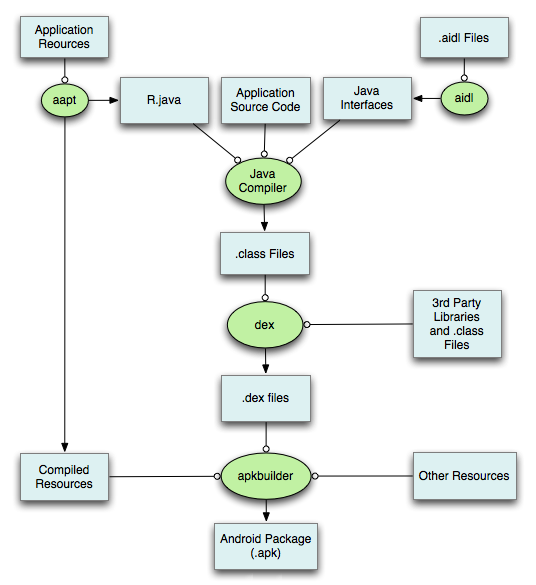
\includegraphics[height=0.8\textheight]{slides/android-application-apk/apk-building-1.png}\\
    {
      \tiny
      Credits: \url{http://developer.android.com}
    }
  \end{figure}
\end{frame}

\begin{frame}
  \frametitle{APK Building}
  \begin{figure}[h!]
    \centering
    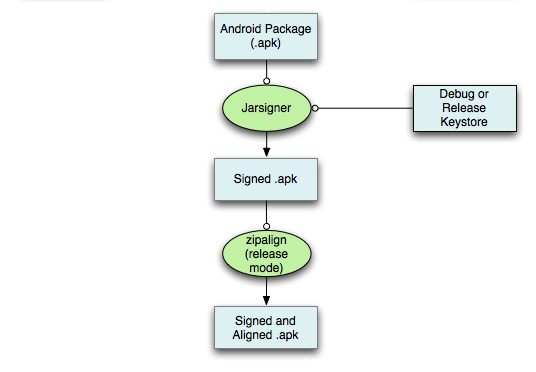
\includegraphics[height=0.8\textheight]{slides/android-application-apk/apk-building-2.png}\\
    {
      \tiny
      Credits: \url{http://developer.android.com}
    }
  \end{figure}
\end{frame}
